\section{Généralités sur l'administration sous Linux}
%Sacha
\subsection{Serveur dédié}

\begin{frame}{Qu'est-ce qu'un serveur ?}

\begin{itemize}
  \item Unité dans un datacenter
  \item Serveur \textit{headless}
  \begin{itemize}
    \item Pas d'écran, ni de clavier, ni de souris
  \end{itemize}
\end{itemize}
  \begin{center} 
      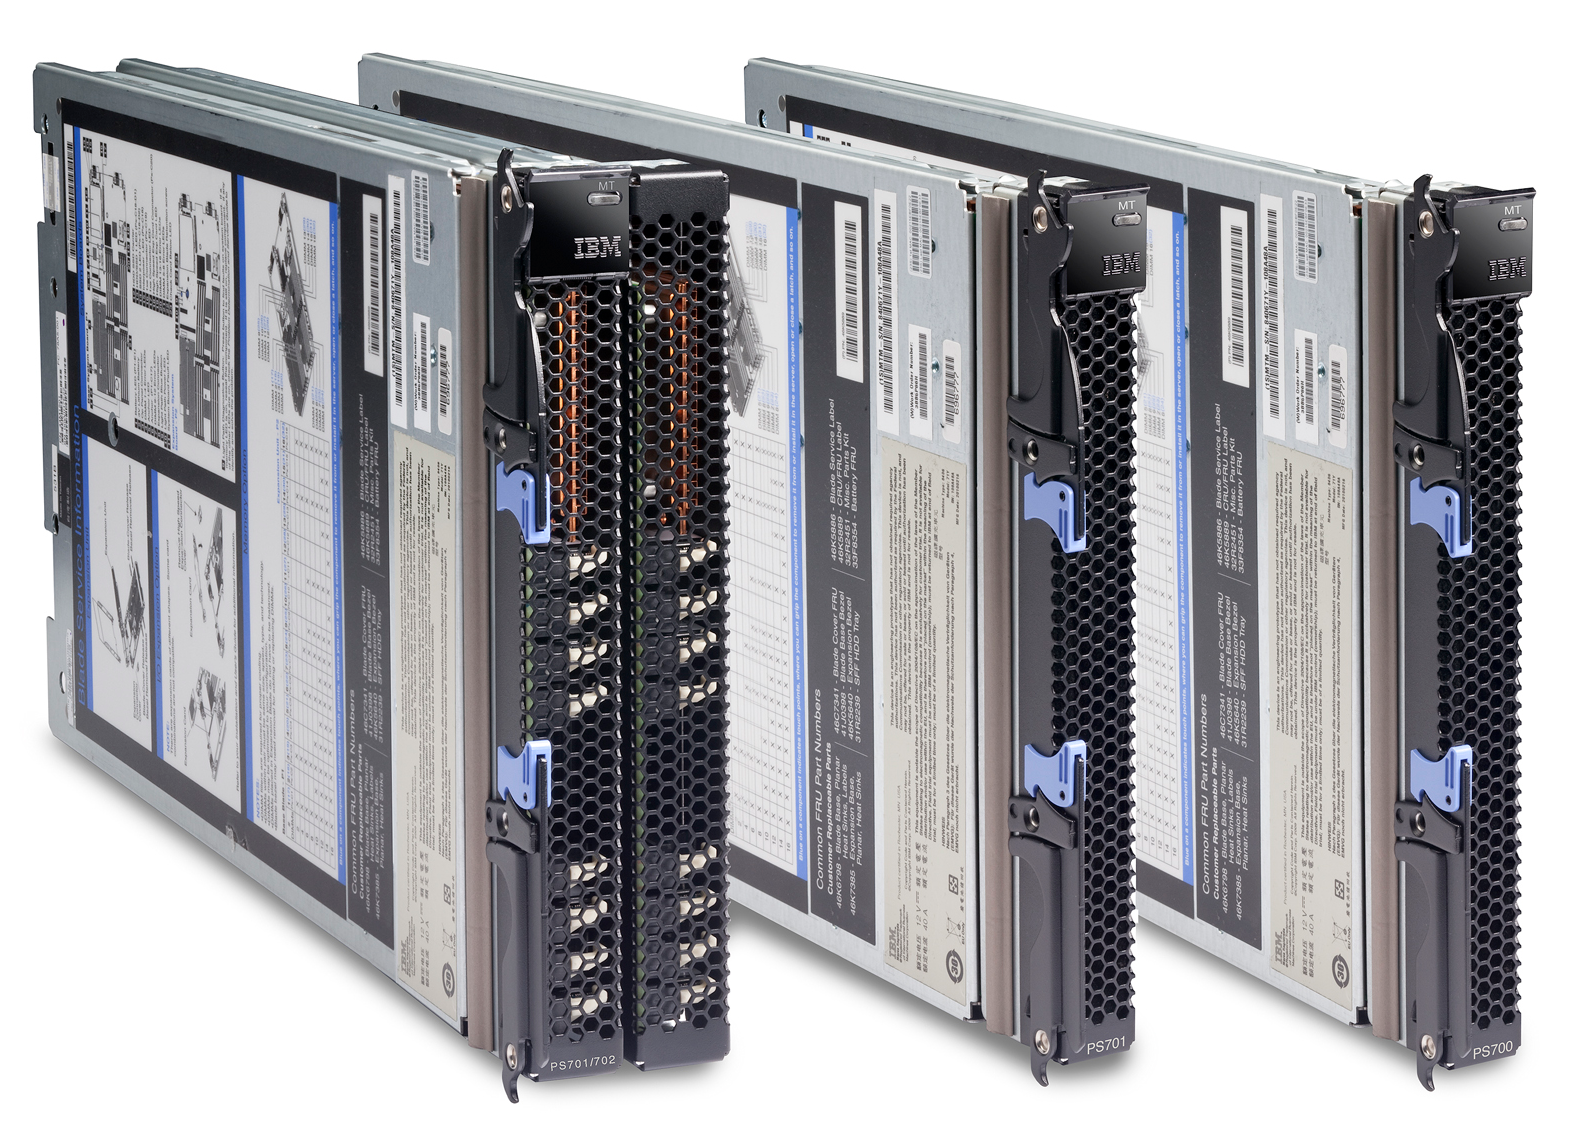
\includegraphics[scale=0.50]{Images/server.png}
  \end{center}

\end{frame}
\begin{frame}{Quel système d'exploitation ?}

\begin{itemize}
  \item Microsoft Windows Server
  \item Linux distribution (Debian, CentOS, Ubuntu Server, etc.)
  \item FreeBSD, Solaris, etc.

\end{itemize}

\end{frame}
\begin{frame}{Pourquoi Linux ?}

\begin{itemize}
  \item Pas d'environnement de bureau
  \begin{itemize}
    \item Administration en ligne de commande (SSH)
    \item Administration web (Webmin, Plesk, GNUPanel, etc.)
  \end{itemize}

\end{itemize}

\end{frame}
\subsection{GNU/Linux}

\begin{frame}{GNU/Linux}

\begin{itemize}
\item Linux est un noyau de système d'exploitation
    \begin{itemize} \item Initié par Linux Torvald \end{itemize}
\item GNU est un système d'exploitation
    \begin{itemize} \item Initié par Richard Stallman \end{itemize}
\item GNU/Linux = GNU over Linux
\end{itemize}

\end{frame}

\frame{\frametitle{GNU/Linux}
		\framesubtitle{Architecture GNU/Linux}
  \begin{center} 
      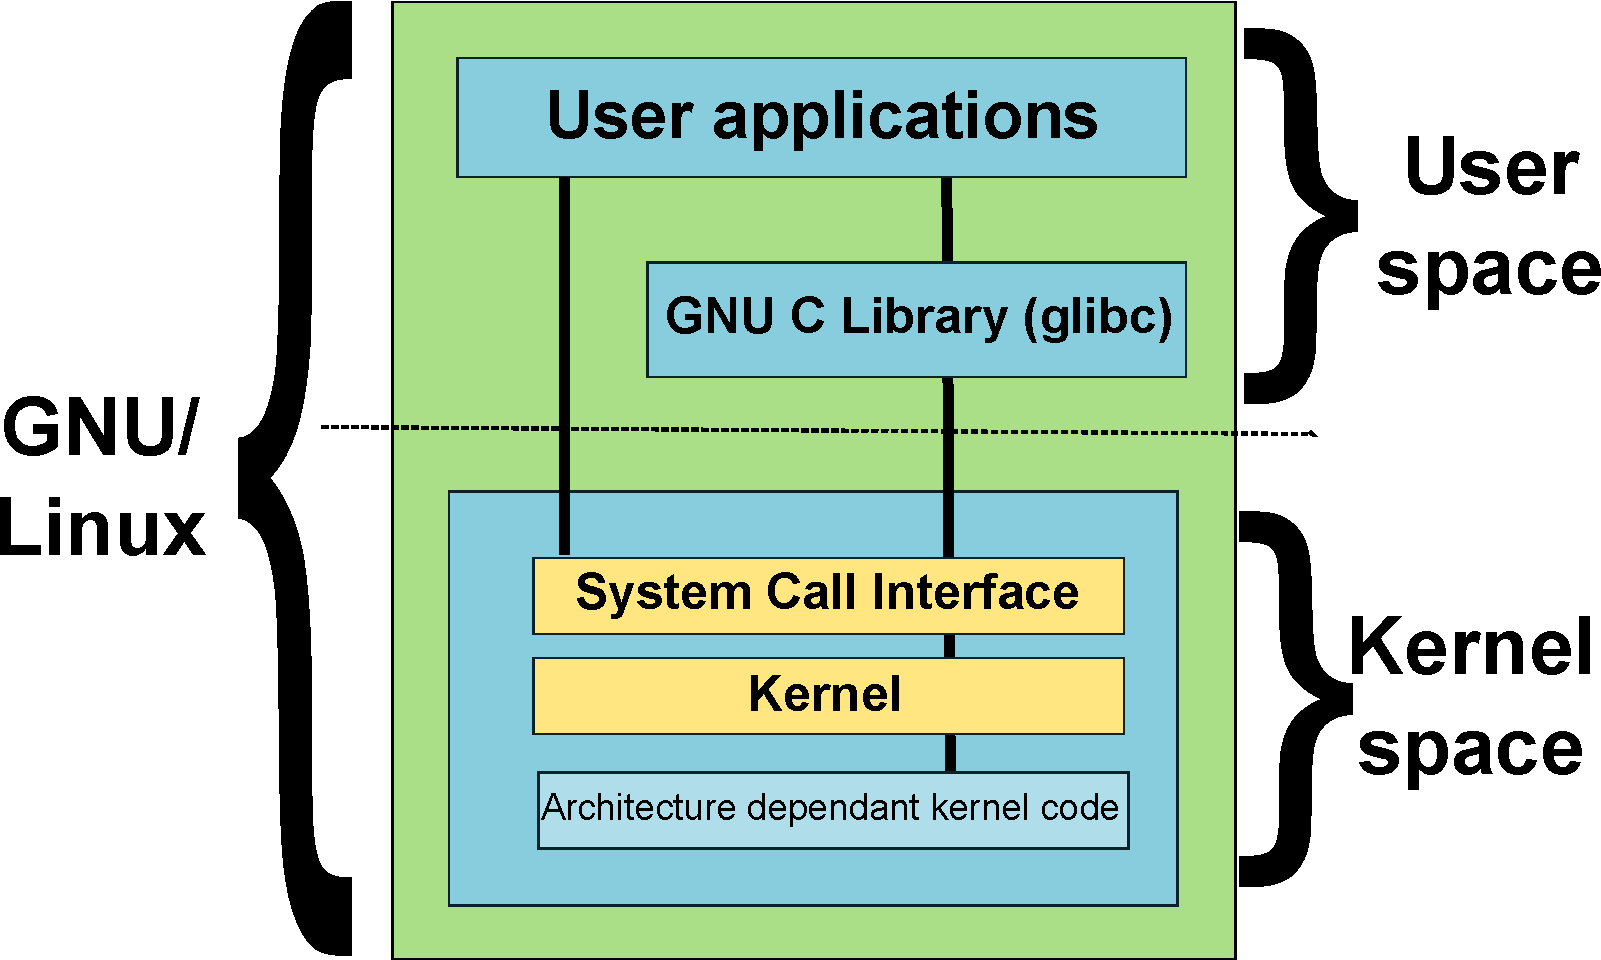
\includegraphics[scale=0.33]{Images/gnulinux.pdf}
  \end{center}
}


\subsection{Distribution linux}
\begin{frame}{Distribution linux}

\begin{itemize}
\item Distribution GNU/Linux = 
\begin{itemize} 
        \item Noyaux Linux + Utilitaire et bibliothèques GNU + ...

        \item Un système d'exploitation composé d'un ensemble de logiciels stable et cohérent  \end{itemize}
\item Trois familles historiques de distributions linux :
  \begin{itemize}
    \item Debian (Debian, Ubuntu, Knopix, etc.)
    \item Slackware (Slackware, S.u.S.E, openSuse, etc.)
    \item Red Hat (Red Hat Enterprise, Mandriva, Fedora, etc...)
  \end{itemize}
\item \href{ldt.pdf}{Linux Distribution Timeline}
\end{itemize}

\end{frame}


\begin{frame}{Commandes de base sous linux}

\begin{itemize}
  \item La documentation : \textbf{man}
  \item Les fichiers
  \begin{itemize}
    \item Navigation (cd, ls)
    \item Édition de fichier (vim, nano, ...)
    \item Gestion des droits (chmod)
  \end{itemize}
  \item Les processus (ps, kill, top, ...)
  \item Les utilisateurs (adduser, deluser, ...)
  \item Les archives (tar, zip, ...)
\end{itemize}

\end{frame}


\begin{frame}{Administration sous debian}

\begin{itemize}
  \item Gestionnaire de packet : apt
    \begin{itemize}
      \item apt-get install <packet>
      \item apt-cache search <nom>
      \item apt-get remove <packet>
    \end{itemize}
  \item Les répertoires systèmes 
  \begin{itemize}
    \item Logs : /var/log
    \item Configuration : /etc/<software>
    \item Gestion des démons : /etc/init.d/<daemon>
  \end{itemize}
\end{itemize}


\end{frame}


